\documentclass[utf8,a4paper,nofonts,9pt]{ctexbook}

\usepackage{amsmath}
\usepackage{xcolor}
\usepackage{hyperref}
\usepackage{graphicx}
\usepackage[many]{tcolorbox}
\usepackage[left=1in, right=1in, top=1in, bottom=1in]{geometry}
% \usepackage[inner=1in, outer=1.25in]{geometry}
\usepackage{titlesec}

\usepackage{src/package/Listings}

\NewDocumentCommand\TODO{m}{\footnote{\textcolor{red}{TODO: #1}}}

\def\dif{\mathop{}\!\mathrm{d}}

\newtcolorbox{exampleBox}{
    sharpish corners, % better drop shadow
    boxrule = 0pt,
    toprule = 4.5pt, % top rule weight
    enhanced,
    fuzzy shadow = {0pt}{-2pt}{-0.5pt}{0.5pt}{black!35} % {xshift}{yshift}{offset}{step}{options} 
}

\setCJKmainfont[Path=../fonts/,BoldFont=SourceHanSerifCN-Bold.otf,ItalicFont=SourceHanSerifCN-Bold.otf]{SourceHanSerifCN-Regular.otf}
\setCJKsansfont[Path=../fonts/,BoldFont=SourceHanSansCN-Bold.otf]{SourceHanSansCN-Regular.otf}
\setCJKmonofont[Path=../fonts/]{SourceHanSansCN-Regular.otf}

\setcounter{secnumdepth}{4}

\titleformat{\paragraph}
{\normalfont\normalsize\bfseries}{\theparagraph}{1em}{}
\titlespacing*{\paragraph}
{0pt}{3.25ex plus 1ex minus .2ex}{1.5ex plus .2ex}

\title{Cookbook}
\author{周泓余\thanks{PeterlitsZo}}

\begin{document}

\maketitle

\tableofcontents
\newpage

%%%%%%%%%%%%%%%%%%%%%%%%%%%%%%%%%%%%%%%%%%%%%%%%%%%%%%%%%%%%%%%%%%%%%%%%%%%%%%%%
%% 数学 %%%%%%%%%%%%%%%%%%%%%%%%%%%%%%%%%%%%%%%%%%%%%%%%%%%%%%%%%%%%%%%%%%%%%%%%
%%%%%%%%%%%%%%%%%%%%%%%%%%%%%%%%%%%%%%%%%%%%%%%%%%%%%%%%%%%%%%%%%%%%%%%%%%%%%%%%
%%%%%%%%%%%%%%%%%%%%%%%%%%%%%%%%%%%%%%%%%%%%%%%%%%%%%%%%%%%%%%%%%%%%%%%%%%%%%%%%
\part{数学}

%%%%%%%%%%%%%%%%%%%%%%%%%%%%%%%%%%%%%%%%%%%%%%%%%%%%%%%%%%%%%%%%%%%%%%%%%%%%%%%%
%% 统计和概率学 %%%%%%%%%%%%%%%%%%%%%%%%%%%%%%%%%%%%%%%%%%%%%%%%%%%%%%%%%%%%%%%%
%%%%%%%%%%%%%%%%%%%%%%%%%%%%%%%%%%%%%%%%%%%%%%%%%%%%%%%%%%%%%%%%%%%%%%%%%%%%%%%%
\chapter{统计和概率学}

%%%%%%%%%%%%%%%%%%%%%%%%%%%%%%%%%%%%%%%%%%%%%%%%%%%%%%%%%%%%%%%%%%%%%%%%%%%%%%%%
%% 随机变量 %%%%%%%%%%%%%%%%%%%%%%%%%%%%%%%%%%%%%%%%%%%%%%%%%%%%%%%%%%%%%%%%%%%%
\section{随机变量}

随机变量是一个定义在样本空间中的实值函数。比如我们令 $Y$ 表示投掷三枚硬币正面朝上的次数,那么 $Y$ 就是一个随机变量,有
\begin{align*}
    P\left\{Y = 0\right\} & = 1 / 8 \\
    P\left\{Y = 1\right\} & = 3 / 8 \\
    P\left\{Y = 2\right\} & = 3 / 8 \\
    P\left\{Y = 3\right\} & = 1 / 8
\end{align*}

对于随机变量 $X$,我们定义它的累积分布函数(简称分布函数)为
\[
    F(x) = P\left\{ X \le x \right\} \quad -\infty < x < \infty
\]

根据随机变量的取值情况,我们可以将随机变量分为离散型随机变量和连续型随机变量。

我们可以使用概率分布列来表示离散型随机变量。随机变量 $X$ 的概率分布列 $p(a)$ 被定义为
\[
    p(a) = P\left\{ X = a \right\}
\]

如果 $X$ 的可能取值构成集合 $\{x_1, x_2, \ldots\}$,那么 $\sum_{i = 1}^\infty p(x_i) = 1$。而分布函数因此可以表示为
\[
    F(a) = \sum_{x \le a} p(x)
\]

因为是离散的,所以对应的分布函数 $F(a)$ 是一个阶梯函数,在 $x_i$ 处有跳跃,跃值为 $p(x_i)$。

%%%%%%%%%%%%%%%%%%%%%%%%%%%%%%%%%%%%%%%%%%%%%%%%%%%%%%%%%%%%%%%%%%%%%%%%%%%%%%%%
%% 期望 %%%%%%%%%%%%%%%%%%%%%%%%%%%%%%%%%%%%%%%%%%%%%%%%%%%%%%%%%%%%%%%%%%%%%%%%
\section{期望}

%% 离散型随机变量的期望 %%%%%%%%%%%%%%%%%%%%%%%%%%%%%%%%%%%%%%%%%%%%%%%%%%%%%%%%
\subsection{离散型随机变量的期望}

对于离散型随机变量 $X$,它的期望记为 $E[X]$,定义为
\[
    E[X] = \sum_{x:\ p(x) > 0} x p(x)
\]

即 $X$ 所有可能取值的一个加权平均。即我们对 $X$ 进行若干次实验后,得到的值的平均值会趋向于 $E[X]$。

进一步地,我们能计算出离散型随机变量的函数 $g(X)$ 的期望。我们可以按照离散型随机变量的期望的定义来计算,即我们先计算出 $g(X)$ 的概率分布列,然后再计算出它的期望。

\begin{exampleBox}
    比如对于离散型随机变量 $X$ 有概率分布列 $p_X( \cdot )$ 如下

    \[
        p_X(-1) = 0.2 \qquad p_X(0) = 0.5 \qquad p_X(1) = 0.3
    \]

    那么 $X$ 的函数 $g(X) = X^2$ 有概率分布列 $p_{g(X)}( \cdot )$ 如下

    \[
        p_{g(X)}(0) = 0.5 \qquad p_{g(X)}(1) = 0.5
    \]

    容易得到 $E[X] = 0.1$,而 $E[X^2] = 0.5$。从这里我们就可以看出来,$(E[X])^2 \ne E[X^2]$。
\end{exampleBox}

我们可以更规范地说,对于 $E[g(X)]$,我们有
\[
    E[g(X)] = \sum_{i} g(x_i) p(x_i)
\]

%% 随机变量和的期望 %%%%%%%%%%%%%%%%%%%%%%%%%%%%%%%%%%%%%%%%%%%%%%%%%%%%%%%%%%%%
\subsection{随机变量和的期望}

不妨假设样本空间 $S$ 是一个有限的或者可数无限的集合。
给定一个随机变量 $X$,则当 $s \in S$ 时,令 $X(s)$ 表示此时随机变量 $X$ 的取值,而 $Y$ 同理,即 $Z = X + Y$ 同样是随机变量,而且 $Z(s) = X(s) + Y(s)$ 成立。

举例来说,我们假设随机试验由抛掷 5 次硬币组成,那么这里的一个样本 $s \in S$ 可能为 $(h, t, h, t, h)$。
而 $X$ 表示前三次抛掷中正面朝上的次数,那么 $X(s) = 2$,而 $Y$ 表示后两次抛掷中正面朝上的次数,那么 $Y(s) = 1$,而 $Z(s) = X(s) + Y(s) = 3$。

令 $p(s) = P(\{ s \})$,因为任意事件 $A$ 可以写为有限个或可数无限个互不相容的事件 $s$ 的和,则
\[
    P(A) = \sum_{s \in A} p(s)
\]

假设随机变量 $X$ 的不同取值为 $x_i ( i \ge 1 )$。对于每一个 $i$,令 $S_i$ 表示 $X$ 等于 $x_i$ 时的事件,即 $S_i = \{ s: X(s) = x_i \}$,那么
\begin{align*}
    E[X] & = \sum_{i} x_i P\{ X = x_i \} = \sum_{i} x_i P(S_i) = \sum_{i} x_i \sum_{s \in S_i} p(s) = \sum_{i} \sum_{s \in S_i} x_i p(s) \\
         & = \sum_i \sum_{s \in S_i} X(s) p(s) = \sum_{s \in S} X(s) p(s)
\end{align*}
即 $E[X]$ 有
\[
    E[X] = \sum_{s \in S} X(s) p(s)
\]

对于随机变量 $X_1, X_2, \cdots, X_n$,记 $Z = \sum_{i = 1}^n X_i$,那么有为
\begin{align*}
    E[Z] & = \sum_{s \in S} Z(s) p(s) = \sum_{s \in S} \left( X_1(s) + X_2(s) + \cdots + X_n(s) \right) p(s) \\
         & = \sum_{s \in S} X_1(s) p(s) + \sum_{s \in S} X_2(s) p(s) + \cdots + \sum_{s \in S} X_n(s) p(s) \\
         & = E[X_1] + E[X_2] + \cdots + E[X_n]
\end{align*}
即,随机变量的和的期望即为随机变量的期望的和。

%%%%%%%%%%%%%%%%%%%%%%%%%%%%%%%%%%%%%%%%%%%%%%%%%%%%%%%%%%%%%%%%%%%%%%%%%%%%%%%%
%% 期望 %%%%%%%%%%%%%%%%%%%%%%%%%%%%%%%%%%%%%%%%%%%%%%%%%%%%%%%%%%%%%%%%%%%%%%%%
\section{方差和标准差}

对于随机变量 $X$ 而言,我们定义方差 $\textrm{Var}(X)$ 为
\[
    \textrm{Var}(X) = E\left[ (X - E[X])^2 \right]
\]

但是我们可以对其进行推导,从而得到一个等价的,但是很有意思的表达,即
\[
    \textrm{Var}(X) = E[X^2] - (E[X])^2
\]
这个推导是很简单的。我们还很容易能够发现,根据方差的定义,方差一定大于等于 $0$,所以能说,对于随机变量,它的平方的期望一定大于等于期望的平方。

对于 $X$ 而言,我们定义它的标准差为
\[
    \textrm{SD}(X) = \sqrt{\textrm{Var}(X)}
\]

%%%%%%%%%%%%%%%%%%%%%%%%%%%%%%%%%%%%%%%%%%%%%%%%%%%%%%%%%%%%%%%%%%%%%%%%%%%%%%%%
%% 离散型随机变量 %%%%%%%%%%%%%%%%%%%%%%%%%%%%%%%%%%%%%%%%%%%%%%%%%%%%%%%%%%%%%%
\section{离散型随机变量}

%% 伯努利随机变量和二项随机变量 %%%%%%%%%%%%%%%%%%%%%%%%%%%%%%%%%%%%%%%%%%%%%%%%
\subsection{伯努利随机变量和二项随机变量}

对于随机变量 $X$,如果它的分布列满足
\begin{align*}
    p(0) & = P\left\{ X = 0 \right\} = 1 - p \\
    p(1) & = P\left\{ X = 1 \right\} = p
\end{align*}
其中 $p \in (0, 1)$,那么我们说 $X$ 为伯努利随机变量。

我们假设我们做了 $n$ 次实验,其中每一次实验结果都可以看成一个独立的伯努利随机变量(实验成功,我们则将其记为 $1$,那么实验成功的概率为 $p(1) = p$),那么最后成功的次数也是一个随机变量,我们记它为参数为 $(n, p)$ 的二项随机变量 $X$,它的分布列为
\[
    p(i) = {n \choose i} p^i (1 - p)^{n - i} \qquad i = 0, 1, \cdots, n
\]

伯努利随机变量是参数为 $(1, p)$ 的特殊二项随机变量。

对于二项随机变量 $X$ 而言,不让认为它的参数为 $(n, p)$,那么有期望为
\begin{align*}
    E[X] & = \sum_{i = 0}^{n} i p(i) = \sum_{i = 1}^{n} i p(i) \\
         & = \sum_{i = 1}^{n} i {n \choose i} p^i (1 - p)^{n - i} \\
         & = \sum_{i = 1}^{n} i {n! \over i! (n - i)!} p^i (1 - p)^{n - i} \\
         & = np \sum_{i = 1}^{n} {(n - 1)! \over (i - 1)! \left[(n - 1) - (i - 1)\right]!} p^{i - 1} (1 - p)^{(n - 1) - (i - 1)} \\
         & = np \sum_{j = 0}^{m} {m! \over j! (m - j)!} p^j (1 - p)^{m - j} \\
         & = np
\end{align*}
这里我们知道 $\sum_{j = 0}^{m} {m! \over j! (m - j)!} p^j (1 - p)^{m - j} = 1$,所以能够知道对于参数为 $(n, p)$ 的二项随机变量 $X$ 而言,$E[X] = np$。

我们可以进一步地解随机变量的次方对应的随机变量 $X^k$ 的期望,有
\begin{align*}
    E[X^k] & = \sum_{i = 1}^{n} i^k {n \choose i} p^i (1 - p)^{n - i} \\
           & = \sum_{i = 1}^{n} i^{k - 1} n {n - 1 \choose i - 1} p^i (1 - p)^{n - i} \qquad \textrm{这里有 $i {n \choose i} = n {n - 1 \choose i - 1}$} \\
           & = np \sum_{i = 1}^{n} i^{k - 1} {n - 1 \choose i - 1} p^{i - 1} (1 - p)^{n - i} \\
           & = np \sum_{j = 0}^{n - 1} (j + 1)^{k - 1} {n - 1 \choose j} p^j (1 - p)^{(n - 1) - j} \\
           & = np E[(Y + 1)^{k - 1}]
\end{align*}
其中 $Y$ 为一个二项随机变量,它的参数为 $(n - 1, p)$。那么有
\begin{align*}
    E[X^2] & = np E[Y + 1] \\
           & = np [(n - 1)p + 1]
\end{align*}
带入到方差的公式中,有
\begin{align*}
    \textrm{Var}(X) = E[X^2] - (E[X])^2 = np [(n - 1)p + 1] - (np)^2 = np (1 - p)
\end{align*}

给出一个重要结论,对于参数为 $(n, p)$ 的二项随机变量 $X$,有
\begin{center}
    \fbox{$ E[X] = np \qquad \textrm{Var}(X) = np (1 - p) $}
\end{center}

此外,我们需要意识到,如果 $X$ 是参数 $(n, p)$ 对应的二项随机变量,那么对于 $k$ 从 $0$ 到 $n$,其 $P\{ X = k \}$ 会先单调递增,然后再单调递减。当 $k$ 为
\[
    \left\lfloor (n + 1) p \right\rfloor
\]
时,$P\{X = k\}$ 取得最大值。

%% 柏松随机变量 %%%%%%%%%%%%%%%%%%%%%%%%%%%%%%%%%%%%%%%%%%%%%%%%%%%%%%%%%%%%%%%%
\subsection{泊松随机变量}

对于随机变量 $X$,如果满足
\[
    p(i) = P\{X = i\} = e^{-\lambda} {\lambda^i \over i!} \qquad i = 0, 1, 2, \ldots
\]
那么我们说 $X$ 是服从参数 $\lambda$ 的泊松随机变量。当 $n$ 足够大,然后 $p$ 又足够小使得 $np$ 保持适当的大小的时候,那么参数为 $(n, p)$ 的二项随机变量可以近似地看为服从 $\lambda = np$ 的泊松随机变量(反过来也成立)。也就是说,对于满足这个条件的二项随机变量 $X$ 有
\begin{align*}
    P\{X = i\} & = {n \choose i} p^i (1 - p)^{n - i} = {n! \over i! (n - i)!} \left( {\lambda \over n} \right)^i \left( 1 - {\lambda \over n} \right)^{n - i} \\
               & = {n (n - 1) \cdots (n - i + 1) \over i!} {\lambda^i \over n^i} {(1 - \lambda / n)^n \over (1 - \lambda / n)^i}
\end{align*}
对于充分大的 $n$ 和适当的 $\lambda$,有\footnote{书中没有指出来,但是我看这第三个表达式的含义恐怕需要 $i$ 也不能太大?似乎因为 $np$ 本身保持适当的值,所以导致 $i$ 取 $np$ 附近的值时,$p(i)$ 的值才会比较大的样子,似乎 $i$ 过大的情况下,$p(i)$ 就会约等于 $0$ 了。}
\[
    \left(1 - {\lambda \over n}\right)^n \approx e^{-\lambda}, \qquad n (n - 1) \cdots (n - i + 1) \approx n^i, \qquad \left(1 - {\lambda \over n}\right)^i \approx 1
\]
那么有
\[
    P\{X = i\} = {\lambda^i \over i!} e^{-\lambda}
\]

举例来说,某页印刷错的字母个数 $X$ 即可以视为泊松随机变量。每个字母印刷错误的概率很小,为 $p$,该页的字母个数为 $n$,那么 $X$ 的参数 $\lambda$ 满足 $\lambda = np$。

我们知道,对于二项随机变量而言,期望和方差分别为 $np$ 和 $np(1 - p)$。因为泊松随机变量可以视为特殊情况下的二项随机变量,所以泊松分布的期望和方差可以带入得到 $\lambda$ 和 $\lambda$(因为 $p$ 很小,所以我们认为 $1 - p$ 可以视为 $1$)。

%% 几何随机变量 %%%%%%%%%%%%%%%%%%%%%%%%%%%%%%%%%%%%%%%%%%%%%%%%%%%%%%%%%%%%%%%%
\subsection{几何随机变量}

考虑独立重复实验中,反复实验,直到实验成功的实验总次数 $X$ 为一个随机变量,那么有
\[
    P\{ X = n\} = (1 - p)^{n - 1} p \qquad n = 1, 2, \cdots
\]
那么我们说 $X$ 是服从参数 $p$ 的几何随机变量。几何随机变量的期望为
\[
    E[X] = {1 \over p}
\]
方差为
\[
    \textrm{Var}(X) = {1 - p \over p^2}
\]

%% 负二项随机变量 %%%%%%%%%%%%%%%%%%%%%%%%%%%%%%%%%%%%%%%%%%%%%%%%%%%%%%%%%%%%%%
\subsection{负二项随机变量}

负二项随机变量是几何随机变量的一个延伸。考虑独立重复实验中,反复实验,直到实验成功 $r$ 次的实验总次数 $X$ 为一个随机变量,那么有
\[
    P\{ X = n \} = \left( { n - 1 \over r - 1 } \right) (1 - p)^{n - r} p^r
\]
我们称 $X$ 是服从参数 $(r, p)$ 的负二项随机变量。

负二项随机变量的期望为
\[
    E[X] = {r \over p}
\]
方差为
\[
    \textrm{Var}(X) = {r(1 - p) \over p^2}
\]

%% 超几何随机变量 %%%%%%%%%%%%%%%%%%%%%%%%%%%%%%%%%%%%%%%%%%%%%%%%%%%%%%%%%%%%%%
\subsection{超几何随机变量}

考虑一个坛子中有 $N$ 个球,其中 $m$ 个白球,$N - m$ 个黑球,从中随机无放回地抽取 $n$ 个球,设随机变量 $X$ 为抽到的白球个数,那么我们说 $X$ 是服从参数 $(n, N, m)$ 的超几何随机变量。那么有
\[
    P\{ X = i \} = {{m \choose i} {N - m \choose n - i} \over {N \choose n}} \qquad i = 0, 1, \cdots, n
\]
这个的表达式是直观的。注,我们定义了 $k < 0$ 或者 $r < k$ 时 $r \choose k$ 等于 $0$。

当 $N$ 和 $m$ 相对 $n$ 而言很大的时候,我们可以认为这个时候是否放回对于结果来说是没有影响的。也就是说,超几何随机变量可以近似地看成二项随机变量。

超几何随机变量的期望为
\[
    E[X] = {nm \over N}
\]
方差为
\[
    \textrm{Var}(X) = {nm \over N}\left[ {(n - 1)(m - 1) \over N - 1} + 1 - {nm \over N} \right]
\]
如果令 $p = m / N$,那么有为
\[
    E[X] = np \qquad \textrm{Var}(X) = np(1 - p){1- {n - 1 \over N - 1}}
\]

%% Zeta 随机变量 %%%%%%%%%%%%%%%%%%%%%%%%%%%%%%%%%%%%%%%%%%%%%%%%%%%%%%%%%%%%%%%
\subsection[zeta 分布]{$\zeta$ 分布}

如果一个随机变量有如下的分布列:
\[
    P\{X = k\} = {C \over k^{\alpha + 1}} \qquad k = 1, 2, \cdots
\]
其中 $\alpha > 0$ 为参数,则称该随机变量为服从 $\zeta$ 分布(或者说 Zipf 分布)。而因为概率之和必然等于 1,所以有:
\[
    C = \left[ \sum_{k = 1}^\infty \left( {1 \over k} \right)^{\alpha + 1} \right]^{-1}
\]

%% 概率密度函数 %%%%%%%%%%%%%%%%%%%%%%%%%%%%%%%%%%%%%%%%%%%%%%%%%%%%%%%%%%%%%%%%
\subsection{概率密度函数}

对于随机变量 $X$,我们说它的概率密度函数 $f_X(x)$ 可以用来描述 $X$ 随机变量能够取某个值的概率大小的函数。也就是说,对于 $\forall -\infty < a < b < \infty$,我们有

$$
P\left[ a < X < b \right] = \int_{a}^{b} f_X(x) \dif{x}
$$

即 $X$ 的取值在 $(a, b)$ 之间的概率正好为概率密度函数在这个区间的积分。

%%%%%%%%%%%%%%%%%%%%%%%%%%%%%%%%%%%%%%%%%%%%%%%%%%%%%%%%%%%%%%%%%%%%%%%%%%%%%%%%
%% 协方差 %%%%%%%%%%%%%%%%%%%%%%%%%%%%%%%%%%%%%%%%%%%%%%%%%%%%%%%%%%%%%%%%%%%%%%
\section{协方差}

我们使用协方差来描述随机变量之间的相关程度。我们定义 $X$ 和 $Y$ 这两个随机变量的协方差为

$$
\textrm{cov}(X, Y) = E\left[ ( X - E[X] ) ( Y - E[Y] ) \right]
$$

如果我们说两个随机变量 $X$ 和 $Y$ 正相关的时候,
那么当 $X$ 大于 $E[X]$ 的时候,一般来说,$Y$ 也大概率大于 $E[Y]$,反之亦然。
带入式子可以看出 $\textrm{cov}(X, Y)$ 是大于 $0$ 的。
所以我们可以反过来用协方差来量化地定义两个随机变量之间的相关性。

%%%%%%%%%%%%%%%%%%%%%%%%%%%%%%%%%%%%%%%%%%%%%%%%%%%%%%%%%%%%%%%%%%%%%%%%%%%%%%%%
%% 连续型随机变量 %%%%%%%%%%%%%%%%%%%%%%%%%%%%%%%%%%%%%%%%%%%%%%%%%%%%%%%%%%%%%%
\section{连续型随机变量}

设 $X$ 为一个随机变量。如果存在一个定义在实数轴上的非负函数 $f$,使得对于任一一个实数集 $B$ 满足
\[
    P\left\{ X \in B \right\} = \int_B f(x) \dif{x}
\]
那么 $X$ 是连续型随机变量。而 $f$ 为随机变量 $X$ 的概率密度函数。而其中 $f$ 一定满足
\[
    1 = P\left\{ X \in (-\infty, +\infty) \right\} = \int_{-\infty}^{+\infty} f(x) \dif{x}
\]

所有关于 $X$ 的概率都可以通过 $f$ 得到,即有
\begin{align*}
    P\left\{ a < X < b \right\} & = \int_a^b f(x) \dif{x} \\
    P\left\{ X = a \right\} & = 0 \\
    P\left\{ X < a \right\} & = P\left\{ X \le a \right\} = F(a) = \int_{-\infty}^a f(x) \dif{x}
\end{align*}

%%%%%%%%%%%%%%%%%%%%%%%%%%%%%%%%%%%%%%%%%%%%%%%%%%%%%%%%%%%%%%%%%%%%%%%%%%%%%%%%
%% 正态分布 %%%%%%%%%%%%%%%%%%%%%%%%%%%%%%%%%%%%%%%%%%%%%%%%%%%%%%%%%%%%%%%%%%%%
\section{正态分布}

我们说一个随机变量 $X$ 服从正态分布,那么我们记为 $X \sim N(\mu, \sigma^2)$。

这里的 $\mu$ 表示期望,$\sigma^2$ 表示方差。正态分布的概率密度函数为:

$$
f(x) = {1 \over \sqrt{2\pi}\sigma} \exp\left(-{(x - \mu)^2 \over 2\sigma^2}\right)
$$

我们将 $X \sim N(0, 1)$ 的随机变量称为标准正态分布。这个时候我们带入有概率密度函数如下:

$$
f(x) = {1 \over \sqrt{2\pi}} \exp\left(-{x^2 \over 2}\right)
$$

另外,对于 $X \sim N(\mu, \sigma^2)$ 而言,我们可以说 $Y = {X - \mu \over \sigma}$ 服从标准正态分布。

在 Rust 中,我们可以通过下面的方式来完成模拟(这里的 \verb|v| 即为一个正态分布的抽样):

\begin{lstlisting}
use rand_distr::{Distribution, Normal};

let normal = Normal::new(0.0, 1.0).unwrap();
let v = normal.sample(&mut rand::rng());
println!("{} is from a N(0, 1) distribution", v);
// 0.8033917292233297 is from a N(0, 1) distribution
\end{lstlisting}

在文档项目中的 \verb|playground| 目录下运行下面的命令即可:

\begin{lstlisting}
cargo run --bin 00_normal
\end{lstlisting}

%%%%%%%%%%%%%%%%%%%%%%%%%%%%%%%%%%%%%%%%%%%%%%%%%%%%%%%%%%%%%%%%%%%%%%%%%%%%%%%%
%% 伊藤引理 %%%%%%%%%%%%%%%%%%%%%%%%%%%%%%%%%%%%%%%%%%%%%%%%%%%%%%%%%%%%%%%%%%%%
\section{伊藤引理}
\label{title:ItosLemma}

[TODO]

%%%%%%%%%%%%%%%%%%%%%%%%%%%%%%%%%%%%%%%%%%%%%%%%%%%%%%%%%%%%%%%%%%%%%%%%%%%%%%%%
%% 标准布朗运动 %%%%%%%%%%%%%%%%%%%%%%%%%%%%%%%%%%%%%%%%%%%%%%%%%%%%%%%%%%%%%%%%
\section{标准布朗运动}

我们这么定义标准布朗运动,对于定义在非负实数(时域)$t$ 上的连续随机过程 $\{B_t, t \ge 0\}$,满足以下条件:

\begin{itemize}
    \item $B(0) = 0$;
    \item 平稳性:对于所有 $0 < s < t$,增量 $B(t) - B(s)$ 符合均值为 $0$,方差为 $t - s$ 的正态分布。
    \item 独立增量:对于所有 $0 \le s < t < u < v$,增量 $B(t) - B(s)$ 和 $B(v) - B(u)$ 是独立的。
\end{itemize}

这个时候我们就说 $B(t)$ 是一个标准布朗运动。

在编程实现中,想要模拟连续的标准布朗运动是不现实且没有必要的,我们可以用离散的方式来模拟。
在 Rust 中,随机数可以通过 \verb|rand| 来生成,但是为了通过正态分布生成随机数,我们还需要使用 \verb|rand_distr|。
我们假设按照单位时间为 1s,那么中国股市的一天的交易时间就一共有 14400 个单位时间(对应 4 个小时)。
我们尝试循环 14400 次,每次都生成单位时间内对应的差 $\Delta B$,并且将其累加到 $B$ 上。
根据标准布朗运动的定义,我们很容易知道 $\Delta B$ 服从一个均值为 0,方差为 1 的标准正态分布(我们定义单位时间的长度就是 $1$)。
然后因为增量都是独立的,所以 $\Delta B$ 的求值和之前的求值无关,这是一个非常优良的特征。这使得下面的代码很容易实现:

\begin{lstlisting}
use rand_distr::{Distribution, Normal};

fn std_brownian_motion(steps: usize) -> Vec<f64> {
    let mut rng = rand::rng();

    let normal = Normal::new(0.0, 1.0).unwrap();
    let mut bm = vec![0.0];

    for _ in 0..steps {
        let v = normal.sample(&mut rng);
        bm.push(bm.last().unwrap() + v);
    }

    bm
}

std_brownian_motion(14400);
\end{lstlisting}

在文档项目中的 \verb|playground| 目录下运行如下命令即可:

\begin{lstlisting}
cargo run --bin 01_std_brownian_motion
\end{lstlisting}

在浏览器中,可以看到标准布朗运动的图像。如图 \ref{fig:stdBrownianMotion} 所示。

\begin{figure}[h]
    \centering
    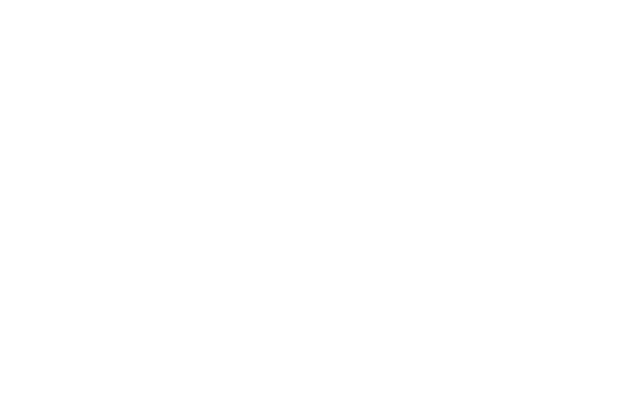
\includegraphics[width=0.8\textwidth]{src/static/00_std_brownian_motion.png}
    \caption{标准布朗运动}
    \label{fig:stdBrownianMotion}
\end{figure}

%%%%%%%%%%%%%%%%%%%%%%%%%%%%%%%%%%%%%%%%%%%%%%%%%%%%%%%%%%%%%%%%%%%%%%%%%%%%%%%%
%% 几何布朗运动 %%%%%%%%%%%%%%%%%%%%%%%%%%%%%%%%%%%%%%%%%%%%%%%%%%%%%%%%%%%%%%%%
\section[几何布朗运动]{几何布朗运动\protect\footnotemark}
\footnotetext{见 \url{https://zhuanlan.zhihu.com/p/38293827}。}

我们可以在标准布朗运动 $B(t)$ 的基础上定义几何布朗运动。在定义之前,我们先定义有漂移的布朗运动 $X(t)$,它有:

$$
\dif{X(t)} = \mu \dif{t} + \sigma \dif{B(t)}
$$

我们知道 $B(t)$ 随机变量在 $t = 1$ 的期望为 $0$,而标准差为 $1$,经过偏移后,$X(t)$ 的期望和方差属性都有所变化。
这里 $\mu$ 被用于表示在单位时间内的期望增长率,而 $\sigma$ 被用于表示单位时间内的标准差。

在量化交易中,我们可以使用这个来描述收益率,而对于股票价格 $S(t)$ 而言,因为有 ${\dif{S(t)} \over S(t)} = \dif{X(t)}$。所以有:

$$
\dif{S(t)} = \mu S(t) \dif{t} + \sigma S(t) \dif{B(t)}
$$

通过伊藤引理 \ref{title:ItosLemma},我们可以得到:

$$
S(t) = S_0 \exp\left(\left(\mu - {\sigma^2 \over 2}\right)t + \sigma B(t)\right)
$$

我们可以使用 Rust 来对齐进行描述:

\begin{lstlisting}
use rand_distr::{Distribution, Normal};

fn geo_brownian_motion(steps: usize, mu: f64, sigma: f64, s0: f64) -> Vec<f64> {
    let mut rng = rand::rng();

    let normal = Normal::new(0.0, 1.0).unwrap();
    let mut bm = vec![s0];

    for _ in 0..steps {
        let z = normal.sample(&mut rng);
        let last_val = bm.last().unwrap();

        let drift = mu - 0.5 * sigma.powi(2);
        let diffusion = sigma * z;
        let new_val = last_val * (drift + diffusion).exp();

        bm.push(new_val);
    }

    bm
}
\end{lstlisting}

在 \verb|playground| 目录下运行如下命令即可:

\begin{lstlisting}
cargo run --bin 02_geo_brownian_motion
\end{lstlisting}

可以在浏览器中看到对应的几何布朗运动的图像。图 \ref{fig:geoBrownianMotion} 展示了几何布朗运动的一个例子。
(在这个图中,我们假定它为一个指数的日内曲线,其中年化收益率为 $8\%$,而一年的方差设置为 $10$)。

\begin{figure}[h]
    \centering
    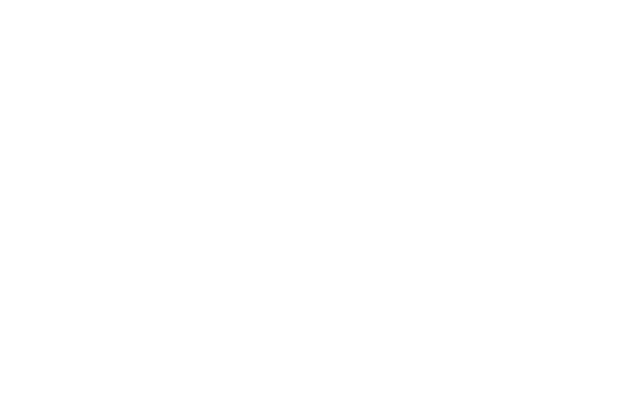
\includegraphics[width=0.8\textwidth]{src/static/01_geo_brownian_motion.png}
    \caption{几何布朗运动}
    \label{fig:geoBrownianMotion}
\end{figure}


%%%%%%%%%%%%%%%%%%%%%%%%%%%%%%%%%%%%%%%%%%%%%%%%%%%%%%%%%%%%%%%%%%%%%%%%%%%%%%%%
%% 金融经济学 %%%%%%%%%%%%%%%%%%%%%%%%%%%%%%%%%%%%%%%%%%%%%%%%%%%%%%%%%%%%%%%%%%
%%%%%%%%%%%%%%%%%%%%%%%%%%%%%%%%%%%%%%%%%%%%%%%%%%%%%%%%%%%%%%%%%%%%%%%%%%%%%%%%
%%%%%%%%%%%%%%%%%%%%%%%%%%%%%%%%%%%%%%%%%%%%%%%%%%%%%%%%%%%%%%%%%%%%%%%%%%%%%%%%
\part{金融经济学}

%%%%%%%%%%%%%%%%%%%%%%%%%%%%%%%%%%%%%%%%%%%%%%%%%%%%%%%%%%%%%%%%%%%%%%%%%%%%%%%%
%% 相关文档 %%%%%%%%%%%%%%%%%%%%%%%%%%%%%%%%%%%%%%%%%%%%%%%%%%%%%%%%%%%%%%%%%%%%
%%%%%%%%%%%%%%%%%%%%%%%%%%%%%%%%%%%%%%%%%%%%%%%%%%%%%%%%%%%%%%%%%%%%%%%%%%%%%%%%
\chapter{相关文档}

证券公司客户交易终端信息处理标准:\url{http://www.cncapital.net/szsa/2023/03/09/e45293b8.pdf}。
还有一个国融证劵的客户终端信息技术规范,但是没找到对应的链接。

%%%%%%%%%%%%%%%%%%%%%%%%%%%%%%%%%%%%%%%%%%%%%%%%%%%%%%%%%%%%%%%%%%%%%%%%%%%%%%%%
%% 金融市场基础知识 %%%%%%%%%%%%%%%%%%%%%%%%%%%%%%%%%%%%%%%%%%%%%%%%%%%%%%%%%%%%
%%%%%%%%%%%%%%%%%%%%%%%%%%%%%%%%%%%%%%%%%%%%%%%%%%%%%%%%%%%%%%%%%%%%%%%%%%%%%%%%
\chapter{金融市场基础知识}

%%%%%%%%%%%%%%%%%%%%%%%%%%%%%%%%%%%%%%%%%%%%%%%%%%%%%%%%%%%%%%%%%%%%%%%%%%%%%%%%
%% 市场 %%%%%%%%%%%%%%%%%%%%%%%%%%%%%%%%%%%%%%%%%%%%%%%%%%%%%%%%%%%%%%%%%%%%%%%%
\section{市场}

交易发生在市场之上。我们可以使用 ISO 10383 来标识一个给定的市场。例如 XSHG 表示
上交所,而 XSHE 表示深交所。这里给出市场列表如下:

\begin{enumerate}
    \item XSHG:(中国)上海证劵交易所,简称上交所;
    \item XSHE:(中国)深圳证劵交易所,简称深交所;
    \item BJSE:(中国)北京证劵交易所,简称北交所;
    \item NEEQ:(中国)全国中小企业股份转让系统;
    \item CCFX:(中国)中国金融期货交易所;
    \item XDCE:(中国)大连商品交易所;
    \item XSGE:(中国)上海期货交易所;
    \item XZCE:(中国)郑州商品交易所;
    \item SHGE:(中国)上海黄金交易所;
    \item CSSX:(中国)上海不锈钢交易所;
    \item XCFE:(中国)中国外汇交易中心;
\end{enumerate}

%% 交易时间 %%%%%%%%%%%%%%%%%%%%%%%%%%%%%%%%%%%%%%%%%%%%%%%%%%%%%%%%%%%%%%%%%%%%
\subsection{交易时间}

其中上交所、深交所、北交所三个交易所的交易时间均采用下面规则\footnote{上交所见《
上海证劵交易所交易规则(2023 年修订)》第 2.4 节,深交所见《深圳证券交易所交易规
则(2023 年修订)》第 2.3 节,北交所见《北京证券交易所交易规则(试行)》第 2.3 
节。}:

\begin{enumerate}
    \item 交易日为周一到周五,法定节假日和交易所公布的休市日除外(此时交易所位于
        休市状态);
    \item 采取竞价交易方式的,每个交易日的 9:15 至 9:25 为开盘集合竞价时间,9:30
        至 11:30、13:00 至 14:57 为连续竞价时间,14:57 至 15:00 为收盘集合竞价时
        间。经中国证监会批准,交易所所可以调整交易时间。交易时间内因故停市,交易
        时间不作顺延。
\end{enumerate}

其中上交所还指定了基金交易的时间,基金交易没有收盘集合竞价时间,相反的,它的交易
时间为 9:15 至 11:30 和 13:00 至 15:00。开市期间停牌并复牌的证劵也可能不遵守本规
则。

%% 交易对象 %%%%%%%%%%%%%%%%%%%%%%%%%%%%%%%%%%%%%%%%%%%%%%%%%%%%%%%%%%%%%%%%%%%%
\subsection{交易对象}

以上交所为例,它可以上市股票、基金、权证、存托凭证和证监会批准的其他交易品种(统
称为证劵),并且能够在市场内挂牌交易。当证劵上市期届满或者依法不具备上市条件的时
候,交易所会终止其上市交易并予以摘牌。对于涉嫌违法违规交易的证卷会实施特别停牌并
予以公告。

%% 标的代码分配 %%%%%%%%%%%%%%%%%%%%%%%%%%%%%%%%%%%%%%%%%%%%%%%%%%%%%%%%%%%%%%%%
\subsection{标的代码分配}

在上交所,标的代码分配可见《上海证券交易所证券交易业务指南第 4 号——证券代码段分
配指南(2022 年第 9 次修订)》文档。

根据文档所诉,标的代码使用 6 位数字来表示。第一位为类别标识,第二到第三位为业务
标识,最后三位为顺序编码。

首位为 0 表示指数和国债。首位为 6 标识 A 股或者存托凭证,首位为 9 标识 B 股。然
后前三位为 000 表示上证指数系列和中证指数系列。前三位为 600、601、603、605 则表
示主板 A 股股票。688 表示科创板。

在深交所,标的代码分配可见《深圳证券交易所数据接口规范(Ver 4.72)》文档第 17
页。

根据文档所诉,我们使用 6 位数字来表示标的代码。其中前三位 000-001 表示主板 A
股。前三位 002-004 为中小企业板股票。前三位为 200-209 为 B 股。300-309 为创业板
股票。

%% 标的名称 %%%%%%%%%%%%%%%%%%%%%%%%%%%%%%%%%%%%%%%%%%%%%%%%%%%%%%%%%%%%%%%%%%%%
\subsection{标的名称}

标的名称一般为简称。在特殊时期会变更以提醒消费者。例如:

\begin{itemize}
    \item 带 DR 标识。表示该标的正在除息除权。
    \item 带 XR 标识。表示该标的正在除权。
    \item 带 XD 标识。表示该标的正在除息。
    \item 带 N 标识。表示该标的为当日新上市。
    \item 带 C 标识。表示该标的为上市次日到第五日。
    \item 带 ST 标识。表示该标的存在风险。其中,名称前缀 “*ST” 表示存在退市风
        险。而 “ST” 则表示存在其他风险。
    \item 带 U 标识。表示该标的暂未盈利。
    \item 带 W 标识。表示该标的发行人具有表决权差异安排。
    \item 带 V 标识。表示该标的发行人具有协议控制架构或者类似特殊安排。
\end{itemize}

%% 申报限制 %%%%%%%%%%%%%%%%%%%%%%%%%%%%%%%%%%%%%%%%%%%%%%%%%%%%%%%%%%%%%%%%%%%%
\subsection{申报限制}

对于上交所的科创板而言(688 开头),其限价申报的申报量不应该小于 200 股,且不超
过 10 万股。市价申报的申报量不应该小于 200 股,且不操作 5 万股。卖出时,余额不足
200 股的部分应当一次性申报卖出。

%%%%%%%%%%%%%%%%%%%%%%%%%%%%%%%%%%%%%%%%%%%%%%%%%%%%%%%%%%%%%%%%%%%%%%%%%%%%%%%%
%% 交易 %%%%%%%%%%%%%%%%%%%%%%%%%%%%%%%%%%%%%%%%%%%%%%%%%%%%%%%%%%%%%%%%%%%%%%%%
\section{交易}

我们在市场上可以交易。一般的标的分为两个方向,分别是买入(bid)或者卖出(ask)。
这里的 “ask” 并非是一种询问,而是一种声明或要求。当卖方想要出手一些标的时,他会
给出一个卖价(ask price),而回应他的买方则会和他达成交易。而 “bid” 则表示愿意为
这个标的出多少钱。

%%%%%%%%%%%%%%%%%%%%%%%%%%%%%%%%%%%%%%%%%%%%%%%%%%%%%%%%%%%%%%%%%%%%%%%%%%%%%%%%
%% 账户 %%%%%%%%%%%%%%%%%%%%%%%%%%%%%%%%%%%%%%%%%%%%%%%%%%%%%%%%%%%%%%%%%%%%%%%%
\section{账户}

用户需要在市场上交易的时候,需要先在券商处开通一个账户。

用户在券商(证券经营机构)开通账户时,其会为办理业务的投资者(个人或者机构)分配
唯一身份标识代码,通常由数字或者数字和字母构成(6 - 12 位编码),这是机构内部标
识客户身份、关联全量业务数据的总索引。客户号需要和投资者真实身份信息(如个人身份
证号、机构统一社会信用代码)绑定,且一个投资者在同一证券经营结构下仅能拥有唯一客
户号。

用户会在券商开立用于管理资金流转的账户,用于存放投资者用户证券交易的资金,并进行
资金的存取、划转、清算、交收等操作。同一投资者在同一卷商下只能开立一个类型的资金
账户。

而证券账户是由中国证券登记结算有限责任公司(以下简称 “中国结算”)统一为投资者开
立的用于登记投资者持有证券的品种、数量、权益变动和相关权益归属的账户。又称为 “股
东账户” 或者 “证券登记账户”。是证券持有和过户的法定载体。

同一个投资者在同一市场最多可以申请开立 3 个 A 股账户、封闭式基金账户,只能申请开
立 1 个信用账户、B 股账户。每个投资者在同一个券商只能开设 1 个有效的 A 股账户。

一个深圳证券账户可以托管多个证券公司同时使用,但是一个上海证券账户仅能指定一家证
券公司使用。

%% 业务流程 %%%%%%%%%%%%%%%%%%%%%%%%%%%%%%%%%%%%%%%%%%%%%%%%%%%%%%%%%%%%%%%%%%%%
\subsection{业务流程}

个人投资者需要先开户才能继续。开户的整个流程为:

\begin{enumerate}
    \item 个人投资者先使用 APP 来申请开户。在 APP 上填写开户请求,提交开户所需资
        料。
    \item APP 会将相关请求代理到券商账户系统。
    \item 券商账户系统会首先进行合规审核。
    \item 当审核通过后,券商交易账户会首先开立交易账户,同时发送请求到中国结算来
        开立一码通账户和证券账户。
    \item 当中国结算返回账户开立成功消息之后,券商账户系统会将证券账户和交易账户
        (资金账户)绑定。
    \item 绑定成功后,它会将结果返回给 APP。同时它会通知集中交易柜台,用于同步账
        户信息,用于交易。
    \item APP 可以通过这个结果来向用户展示账户信息。
    \item APP 自研柜台可以通过每日上场的方式和集中交易柜台交互来获取账户信息。
\end{enumerate}

%%%%%%%%%%%%%%%%%%%%%%%%%%%%%%%%%%%%%%%%%%%%%%%%%%%%%%%%%%%%%%%%%%%%%%%%%%%%%%%%
%% 股票 %%%%%%%%%%%%%%%%%%%%%%%%%%%%%%%%%%%%%%%%%%%%%%%%%%%%%%%%%%%%%%%%%%%%%%%%
\section{股票}

%% ST %%%%%%%%%%%%%%%%%%%%%%%%%%%%%%%%%%%%%%%%%%%%%%%%%%%%%%%%%%%%%%%%%%%%%%%%%%
\subsection{ST}

ST 股票是指特殊处理的股票。

其中,名称前缀 “*ST” 表示存在退市风险。而 “ST” 则表示存在其他风险。

%%%%%%%%%%%%%%%%%%%%%%%%%%%%%%%%%%%%%%%%%%%%%%%%%%%%%%%%%%%%%%%%%%%%%%%%%%%%%%%%
%% 证劵投资基金 %%%%%%%%%%%%%%%%%%%%%%%%%%%%%%%%%%%%%%%%%%%%%%%%%%%%%%%%%%%%%%%%
\section{证劵投资基金}

投资基金是通过向投资者募集资金,由专业投资机构(基金管理人)进行资金投资和管理,
由基金托管人来进行资金托管。比如如果我们购买 “深证50ETF易方达” 这个 ETF 基金,那
么我们就是投资者,而管理人 “易方达基金” 会负责使用我们的钱来进行投资,并管理对应
的资产,资金不会直接放在 “易方达基金” 中,而是放在托管人 “国泰君安” 中。投资基金
可以分为证劵投资基金和另类投资基金。

根据地区不同,证劵投资基金的名称也有所不同,比如在其他国家或地区,它被称为共同基
金、单位信托基金、集合投资基金或集合投资计划等。

%% 特殊类型基金 %%%%%%%%%%%%%%%%%%%%%%%%%%%%%%%%%%%%%%%%%%%%%%%%%%%%%%%%%%%%%%%%
\subsection{特殊类型基金}

\subsubsection{交易所交易基金(ETF)}

ETF 是 Exchange Traded Fund 的缩写,交易所交易基金是一种在证券交易所上市交易的、
份额可变的投资基金。它结合了封闭式基金和开放式基金的特点。它的最大特点是实物申购
和赎回机制。即它的申购是用一篮子股票或者债卷来换取 ETF 份额,而赎回是用 ETF 份额
换回一篮子股票或者债卷。所以 ETF 有 “最小申购、赎回” 份额的规定,这个单位一般是
30 万份、50 万份或者 100 万份。而申购和赎回必须是这个单位的整数倍。而只有机构投
资者才有能力在一级市场进行申购和赎回,散户只能在二级市场上进行交易。

%%%%%%%%%%%%%%%%%%%%%%%%%%%%%%%%%%%%%%%%%%%%%%%%%%%%%%%%%%%%%%%%%%%%%%%%%%%%%%%%
%% 指数 %%%%%%%%%%%%%%%%%%%%%%%%%%%%%%%%%%%%%%%%%%%%%%%%%%%%%%%%%%%%%%%%%%%%%%%%
\section{指数}

指数可以用来反应多个股票的价值的一个数据。

在中国,一般是由两个公司来完成指数的编制,一个是中证指数有限公司(China
Securities Index Co., Ltd.),另一个是深圳证劵信息有限公司(Shenzhen Securities
Information Co., Ltd.)。其中中证指数有限公司是由上交所和深交所共同成立的。而深
圳证劵信息公司是深交所下属。

中证指数有限公司编制的指数系列包括中证系列指数和上证系列指数。前者的样本空间为沪
市和深市,而后者只包含沪市。而深圳证劵信息公司编制的指数系列彪悍深证系列指数和国
证系列指数。前者的样本空间为深市,而后者为沪市和深市。

指数的计算方法并不简单。以道琼斯指数为例。它的点位 $P$ 可以通过成份股的价格
$P_i$(即第 $i$ 个成份股的价格)和除数 $D$ 来计算:
\[
    P = {\sum_{i} P_i \over D}
\]
但是这种计算方式会因为股份拆分、合并或者成份股列表变动的原因导致 $P$ 发生变动。
为此,除数 $D$ 会进行调整,使得即使发生了变动,变动前和变动后的 $P$ 也不会变动。
这个方式非常简单,但是如果某个成份股即使市值不大,但是因为股本较少而导致股价较
高,这种高价股的波动会非常容易影响到指数点位。

除了道琼斯指数这种价格加权指数计算方式外,我们还有市值加权指数计算方式和等权重指
数等计算方式。

%%%%%%%%%%%%%%%%%%%%%%%%%%%%%%%%%%%%%%%%%%%%%%%%%%%%%%%%%%%%%%%%%%%%%%%%%%%%%%%%
%% 期货 %%%%%%%%%%%%%%%%%%%%%%%%%%%%%%%%%%%%%%%%%%%%%%%%%%%%%%%%%%%%%%%%%%%%%%%%
\section{期货}

一般而言我们交易的期货分为商品期货和金融期货。

%% 交易规则 %%%%%%%%%%%%%%%%%%%%%%%%%%%%%%%%%%%%%%%%%%%%%%%%%%%%%%%%%%%%%%%%%%%%
\subsection{交易规则}

\subsubsection{保证金制度}

在期货交易中,买方和卖方必须按照所买卖期货合约价格的一定比率缴纳资金。例如沪深
300 股指期货交易交易所保证金为 10\%。那么对于 2021 年 3 月交割的沪深 300 股指期
货合约(我们使用符号 IF2103 来表示),如果在某个特定时间点上,它的当前指数点位为
5400 点,而合约乘数位每点 300 元,则一手 IF2103 合约价值,就是当前的指数的指数点
数,乘以合约乘数,即 $1,620,000$ 元。不过,交易中,我们不需要有这么多钱来购入该
期货,我们只需要缴纳保证金,就可以拥有它。保证金比例由交易所规定,如前所属,它是
10\%,所以对应保证金为 $162,000$ 元。也就是说,我们只需要账面上有 $162,000$ 元,
就可以在那个时间点上进行一手 IF2103 的交易。

\subsubsection{双向交易机制}

交易者参与交易分为两种方向,即做多或者做空。做多即认为资产价格未来上涨,那么可以
先买入再卖出。做空即认为资产价格未来下跌,那么可以先卖出再买入。

\subsubsection{T+0 交易制度}

期货交易采用 T+0 交易制度,即在交易日内可以多次买入和卖出。对应的其他标的可能就
是使用 T+1 交易制度,即当天买入的标的只能在下一个交易日卖出。

%% 金融期货 %%%%%%%%%%%%%%%%%%%%%%%%%%%%%%%%%%%%%%%%%%%%%%%%%%%%%%%%%%%%%%%%%%%%
\subsection[金融期货]{金融期货\protect\footnotemark}
\footnotetext{见 \url{https://www.investor.org.cn/learning_center/gmjytx/bk/kj/jyxl_3469/202302/P020230227568934703121.pdf}。}

金融期货是指以金融资产为标的物的期货合约。比如国债期货、股指期货、外汇期货等。

对于商品期货而言,我们通过 “交割” 来将期货价格和现货价格联系了起来。
比如,如果在交割日的时候,期货价格高于现货价格,那么就会有套利者通过买入现货,然后再交割给期货市场的多头。
反之,如果期货价格低于现货价格,那么就会有套利者通过和期货市场的空头完成交割来获得商品,再在现货市场上卖出来获利。

但是在金融期货市场中,我们的确存在标的是可交割的,比如国债期货。这种交割方式和商品期货类似,为实物交割。
但是对于不可交割的标的,我们则会使用另外一种方式来完成交割,这种方式叫做现金交割。
例如股指期货就采用现金交割的方式。

%            date    open    high     low   close  volume   hold  settle
% 0    2024-04-22  3480.8  3513.0  3474.2  3481.0    2078   2042     0.0
% 1    2024-04-23  3481.0  3491.0  3453.6  3460.0    1838   2407     0.0
% 2    2024-04-24  3473.0  3481.2  3453.0  3477.2    1846   3058     0.0
% 3    2024-04-25  3472.0  3500.8  3460.0  3485.0    1788   3721     0.0
% 4    2024-04-26  3490.6  3557.4  3490.6  3548.0    2788   4770     0.0
% ..          ...     ...     ...     ...     ...     ...    ...     ...
% 159  2024-12-16  3940.0  3940.0  3901.2  3911.4   65026  96215     0.0
% 160  2024-12-17  3907.0  3962.0  3907.0  3922.4   89943  89729     0.0
% 161  2024-12-18  3941.4  3959.4  3931.6  3940.2   65404  66736     0.0
% 162  2024-12-19  3910.8  3956.6  3897.2  3944.8   55685  43675     0.0
% 163  2024-12-20  3937.0  3957.6  3921.0  3935.0   31716  19435     0.0
对于股指期货而言,它的标准化合约会规定 “合约乘数” 这一属性。例如沪深 300 股指期货合约的合约乘数被中金所规定为 300。
例如,假设当前沪深 300 股指期货的点位为 3500 点时,一份合约价格就是 $3,500 \times 300 = 1,050,000$ 元(一份合约就价值上百万了)。
比如标的 IF2412 就是一个沪深 300 股指期货,它在 2024/04/22 的时候上市,在 2024/12/20 到期。
标的 IF2412 在 2024/04/22 开盘的时候的价格为 3480.8,这个表示市场在开盘的时候预期认为在 2024/12/20 到期的时候,沪深 300 指数的点位会在 3480.8 点左右。
在 IF2412 交割日那天,它的收盘点位为 3935.0 点位,中金所会计算出未平仓账户的仓位,并根据多头和空头的仓位来计算出现金交割的金额。
双方会通过划转现金的方式来完成交割。例如多头 A 持有一份认购合约,其中合约规定的点位是 $3900.0$,那么在交割的时候,他会收到 $(3935.0 - 3900.0) \times 300 = 10,500$ 元的现金。
这个交割的现金正好等于他以 $3900.0 \times 300$ 买入了一份虚拟的 “沪深 300 指数金融资产”,并以 $3935.0 \times 300$ 卖出这份虚拟的 “沪深 300 指数金融资产” 的差价。
虽然实际上从头到尾并没有这个资产,但是通过现金交割的方式,双方获得投资收益或者对应的损失。
可以看到,即使是不可交割的金融期货合约,也可以通过现金交割的方式来交割,从而将期货价格和现货价格联系起来。

%% 永续期货合约 %%%%%%%%%%%%%%%%%%%%%%%%%%%%%%%%%%%%%%%%%%%%%%%%%%%%%%%%%%%%%%%%
\subsection{永续期货合约}

对于传统的期货而言,我们一般会规定特定的交割日期和交割地点。
但是永续期货合约却没有交割日期和交割地点的限制。
一般只有虚拟数字资产,比如 BTC/USDT、ETH/USDT 等采用永续期货合约。

对于传统期货而言,我们使用交割的方式(包括实物交割和现金交割)来将期货价格和现货价格联系在一起。
但是对于永续合约而言,由于交割的缺失,我们需要另外一个机制使得现货价格和期货价格能够联系在一起。

为此,“资金费用” 作为永续合约的一个关键机制被引入进来了。
它要求多头和空头定期地完成资金划转。对于虚拟货币而言,定期一般指每 4 或 8 小时一次。
当永续期货合约的期货价值大于此时的现货价值时,资金费率为正,此时多头需要向空头支付资金费用。
反之,资金费率为负,此时则需要空头向多头支付费率。

对于币安而言,资金费率 $F$ 受到溢价指数 $P$ 和固定利率 $I$ 影响。其中 $I$ 一般为每日 $0.03\%$。
而如果每 8 小时结算一次,那么每个周期的 $I$ 即为 $0.01\%$。
而溢价指数则是一个动态变量,用于反映期货价格和现货价格之间的差异。
$F$ 的计算公式为:
\[
    F = P + \textrm{clamp}\left( I - P, -0.05\%, 0.05\% \right)
\]
这里的固定利率 $I$ 用于描述传统期货中的持有成本。

而溢价指数 $P$,如前所诉,用于反映期货价格和现货价格之间的差异。
它受到冲击买价 $B$、冲击卖价 $S$ 和指数价格 $M$ 的影响。
指数价格 $M$ 被用于表示标的的现货价值,其为多个交易所现货加权均值计算而得到。
而冲击买卖价 $B$ 和 $S$ 则深层次地表明了市场深度的流动性成本。
它通过模拟吃掉一定深度订单后市场的成交均价,从而揭露市场真实的承受能力。
$P$ 的计算公式为:
\[
    P = {\textrm{max}(0, B - M) - \textrm{max}(0, M - S) \over M}
\]
理想情况下,冲击买价 $B$ 应该大于指数价格 $M$,冲击卖价 $S$ 应该小于指数价格 $M$(否则存在套利空间)。
那么在这种情况下,溢价指数 $P$ 就取决于冲击买价相比于指数价格的偏移 $B - M$ 和冲击卖价相比于指数价格的偏移 $M - S$ 谁更大一些。

%%%%%%%%%%%%%%%%%%%%%%%%%%%%%%%%%%%%%%%%%%%%%%%%%%%%%%%%%%%%%%%%%%%%%%%%%%%%%%%%
%% 加密货币 %%%%%%%%%%%%%%%%%%%%%%%%%%%%%%%%%%%%%%%%%%%%%%%%%%%%%%%%%%%%%%%%%%%%
\section{加密货币}

加密货币是一种数字货币。

对于普通的标的而言,我们可以使用其交易所指定的货币进行交易。例如在上交所上市的股票,我们可以使用人民币来完成交易。但是在加密货币交易所中,我们不会使用这种法定货币来进行交易,而是使用加密货币来进行交易。
所以在交易前,我们需要将人民币等币种兑换成加密货币(比如 USDT),然后再使用这个加密货币来进行交易。
我们可以使用多种加密货币来完成交易。所以在加密货币交易所中,我们会有加密货币对的概念,比如 ETH/BTC 交易对,就表示有用户愿意用 BTC 来购买 ETH,而又有用户愿意用 ETH 来购买 BTC。

举例来说,在币安交易所中,就有交易对 BTC/USDT。

%%%%%%%%%%%%%%%%%%%%%%%%%%%%%%%%%%%%%%%%%%%%%%%%%%%%%%%%%%%%%%%%%%%%%%%%%%%%%%%%
%% 投资术语 %%%%%%%%%%%%%%%%%%%%%%%%%%%%%%%%%%%%%%%%%%%%%%%%%%%%%%%%%%%%%%%%%%%%
%%%%%%%%%%%%%%%%%%%%%%%%%%%%%%%%%%%%%%%%%%%%%%%%%%%%%%%%%%%%%%%%%%%%%%%%%%%%%%%%
\chapter{投资术语}

%%%%%%%%%%%%%%%%%%%%%%%%%%%%%%%%%%%%%%%%%%%%%%%%%%%%%%%%%%%%%%%%%%%%%%%%%%%%%%%%
%% 仓位 %%%%%%%%%%%%%%%%%%%%%%%%%%%%%%%%%%%%%%%%%%%%%%%%%%%%%%%%%%%%%%%%%%%%%%%%
\section{仓位}

当投资者开始进入市场并交易的时候,投资者手上会得到一些资产。
这些投资者持有交易合约或资产数量,即为投资者的持仓。

而仓位,即为投资者持仓相对于其投资账户的总资金的比例。投资者可能会具有多个投资账户。

仓位管理是交易者决定入市交易的时候,对于建仓、加仓、减仓和清仓的计划和管理。

例如我们打算用 10 万元用于交易,其中买入了 3 万元币种,对应 300 单位 BTC 加密货币\footnote{注意,现在不可能有这么便宜的 BTC 了。}。
那么这个时候仓位就是 30\%,或者说 3 层仓(一层对应于 10\%)。
买入的行为叫做开仓或者建仓。
根据仓位的情况,我们可以说我们的仓位是半仓、轻仓、重仓等。
建仓后再次买入叫做加仓,卖出叫做减仓。
全部卖出叫做清仓,持有但是暂时不卖出叫持仓,总是保留部分仓位不进行操作叫做底仓。全部卖出不再买入叫空仓。

在交易过程中我们可能有“保证金”这一概念。
交易者可以通过向经纪人借入资金来放大回报。对应的,交易者需要拿出一部分资产作为抵押,这个抵押即为保证金。
保证金一般用在期货交易中。

另外,对于期货等这种市场允许我们卖空等标的而言,我们的持仓量可正可负。
例如当我们参与期货交易的时候,我们可以卖出一手期货合约,这个时候我们的持仓量为 -1 手。

对于某一标的,我们能计算出该标的的持仓成本。
假设我们成交了 $N_b$ 笔买入订单,$N_s$ 笔卖出订单。
其中第 $i$ 笔订单的成交价格为 $P_i$,每笔订单的成交量为 $Q_i$。
令 $B$ 为买入订单的集合,$S$ 为卖出订单的集合。
那么持仓成本 $C$ 可以通过下面的公式计算:
\[
    C = { \sum_{i \in B} P_i Q_i - \sum_{j \in S} P_j Q_j \over \sum_{i \in B} Q_i - \sum_{j \in S} Q_j }
\]

%%%%%%%%%%%%%%%%%%%%%%%%%%%%%%%%%%%%%%%%%%%%%%%%%%%%%%%%%%%%%%%%%%%%%%%%%%%%%%%%
%% 盈亏 %%%%%%%%%%%%%%%%%%%%%%%%%%%%%%%%%%%%%%%%%%%%%%%%%%%%%%%%%%%%%%%%%%%%%%%%
\section{盈亏}

当我们交易的时候,我们一般会区分两种盈亏,一个是未实现盈亏,一个是已实现盈亏。

未实现盈亏(unrealized profit and loss,UPL)是指交易者持有的仓位在当前市场价格下的盈亏情况。
它即我们将所有未平仓的标的物立即平仓后得到的利润和损失。未实现盈亏又称为浮动盈亏(floating profit and loss,FPL)。
因为它会随着市场行情的不断变化而变化。

已实现盈亏(realized profit and loss,RPL)是指交易者已经完成交易得到的利润或损失。

%%%%%%%%%%%%%%%%%%%%%%%%%%%%%%%%%%%%%%%%%%%%%%%%%%%%%%%%%%%%%%%%%%%%%%%%%%%%%%%%
%% 权益 %%%%%%%%%%%%%%%%%%%%%%%%%%%%%%%%%%%%%%%%%%%%%%%%%%%%%%%%%%%%%%%%%%%%%%%%
\section{权益}

权益(equity)是指投资者在交易账户中的资金总额。
以期货交易为例,权益包含了投资者的初始保证金、追加保证金、已实现盈亏和未实现盈亏。

%%%%%%%%%%%%%%%%%%%%%%%%%%%%%%%%%%%%%%%%%%%%%%%%%%%%%%%%%%%%%%%%%%%%%%%%%%%%%%%%
%% 订单 %%%%%%%%%%%%%%%%%%%%%%%%%%%%%%%%%%%%%%%%%%%%%%%%%%%%%%%%%%%%%%%%%%%%%%%%
\section{订单}

订单(order)是指投资者向交易所或经纪人发出的买入或卖出指令。

订单可以分为市价单、限价单和条件单。
市价单会按照当前的最优价格立即成交。而限价单会根据限定的价格或者更优价格成交。
条件单,比如 OCO 订单会同时设置两个条件,当市场价格低于某个值时买入,或者高于某个值时卖出,
如果一个成立了,那么另一个就会被取消。

在《证券期货业场外市场交易系统接口:第 2 部分:订单接口》文档%
\footnote{见 \url{https://www.sse.com.cn/lawandrules/regulations/csrcannoun/c/10117405/files/7a5d6a32eb854b7d92954f2766db68a3.pdf}。}%
中,订单的状态被分为:

\begin{enumerate}
    \item 新(New)- 新创建的订单,已经提交到系统,但是还没有处理。
    \item 部分成交(Partially Filled)- 一部分成交了。
    \item 已成交(Filled) - 完全成交。
    \item 部分撤销(Done for day)- 撤掉了未完成的部分,但是有一部分已经完成了。
    \item 全部撤销(Canceled)- 完全撤销。
    \item 待撤销(Pending Cancel)- 撤单请求已发出,等待交易所确认。
    \item 已终止(Stopped)- ???。
    \item 已拒绝(Rejected)- ???。
    \item 已延缓(Suspended)- ???。
    \item 待处理(Pending New)- 订单已经提交到交易所,等待交易所确认接受。
    \item 已计算(Calculated)- ???。
    \item 已过期(Expired)- ???。
    \item 已接受(Accepted for bidding)- ???。
    \item 待替换(Pending Replace)- ???。
    \item 非交易订单已接收(Non-trading order has been received)- ???。
\end{enumerate}

%%%%%%%%%%%%%%%%%%%%%%%%%%%%%%%%%%%%%%%%%%%%%%%%%%%%%%%%%%%%%%%%%%%%%%%%%%%%%%%%
%% 标的属性 %%%%%%%%%%%%%%%%%%%%%%%%%%%%%%%%%%%%%%%%%%%%%%%%%%%%%%%%%%%%%%%%%%%%
%%%%%%%%%%%%%%%%%%%%%%%%%%%%%%%%%%%%%%%%%%%%%%%%%%%%%%%%%%%%%%%%%%%%%%%%%%%%%%%%
\chapter{标的属性}

%%%%%%%%%%%%%%%%%%%%%%%%%%%%%%%%%%%%%%%%%%%%%%%%%%%%%%%%%%%%%%%%%%%%%%%%%%%%%%%%
%% 标的代码 %%%%%%%%%%%%%%%%%%%%%%%%%%%%%%%%%%%%%%%%%%%%%%%%%%%%%%%%%%%%%%%%%%%%
\section{标的代码}

一般来说,标的代码是一个唯一的标识符,用于标识一个特定的交易标的。
标的代码由交易所分配,在沪深北市场中,它为 6 位数字。
在其他市场中,标的代码可能会有不同的长度和格式(例如,在港交所中,它是 5 位数字,在其他市场中,存在字母)。

比如 302132 为 “中航成飞” 的标的代码。

%%%%%%%%%%%%%%%%%%%%%%%%%%%%%%%%%%%%%%%%%%%%%%%%%%%%%%%%%%%%%%%%%%%%%%%%%%%%%%%%
%% 市盈率 %%%%%%%%%%%%%%%%%%%%%%%%%%%%%%%%%%%%%%%%%%%%%%%%%%%%%%%%%%%%%%%%%%%%%%
\section{市盈率}

市盈率是市价盈利比率(price earnings ratio,P/E)的简称。

我们在 \ref{title:DDM} 节中讨论了 DDM 模型,它指出了股票的价格取决于其预期分红。而企业往往在盈利后才会有分红。
所以为了给股票估值,那么我们往往会研究这个股票估值指标,即市盈率。它的值是股票价格和每股盈利的比值。
而每股盈利则是公司总盈利除以公司的总股份数。

注意到公司不会将所有盈利都用来分红,公司往往会将一部分盈利拿来用以分红,那么将这个比例记为 $k$,第 $t$ 期的每股分红 $D_t$ 和每股盈利 $E_t$ 有

$$
E_t = kD_t
$$

将其带入到 \ref{title:DDM} 节中的戈登股利增长模型中有

$$
{S_0 \over E_1} = {k \over r - g}
$$

这里的左式即为市盈率。即市盈率取决于分红率、贴现率和盈利增速这三个变量。

这说明了即使一个企业的每股盈利较高,但是如果企业以较低分红率分红的话,投资者也不会愿意投资这个企业。
同样,盈利增速也是一个非常重要的因素,它即使发生的是一点点变化,也会大幅度影响 P/E 的值。

\begin{exampleBox}
如果我们说一个股票的 P/E 为 10,而每股盈利为 10 元的话,那么可以说这个公司的股价在理论上应该为 100 元。
如果我们说因为某种原因,导致了预期的盈利增速 $g$ 发生了变化(比如政策倾斜),即使这个公司在短期内每股盈利不变,但是也会导致市盈率大幅上涨,从而导致价格也大幅上涨。
比如如果 $r = 20\%$,而 $g = 16\%$ 上涨到了 $g' = 18\%$,这个 $2\%$ 的上涨会导致 P/E 翻倍,最后导致股票价格也翻倍。
\end{exampleBox}

\begin{exampleBox}
和上一个例子一样,我们假设 $S_0 = 100$,$E_1 = 10$,$k = 40\%$,$g = 16\%$ 以及 $r = 20\%$,我们来计算投资者在第 0 期买入,到第 1 期卖出得到的回报率。
可以知道投资回报率为

$$
{D_1 + S_1 \over S_0} - 1
$$

即一期得到的分红以及股票价格之和相比一开始的股票价格的涨幅。
我们知道 $D_1 = k E_1 = 4$,而 $S_1 = {D_2 \over r - g} = {D_1 (1 + g) \over r - g} = 116$,所以有

$$
{4 + 116 \over 100} - 1 = 20\% = r
$$

可以知道市场的投资回报率为 $r = 20\%$。这个不难证明。所以贴现率即为投资者所能接受且理论上能获得的回报率(如果实际产生的回报率高于贴现率,那么对这个股票的需求就会上涨,导致价格上涨,进而拉低回报率,最后达到均衡)。
\end{exampleBox}

在实践中,我们一般使用滚动市盈率(trailing P/E)来表示市盈率,即市盈率 TTM,其中 TTM 表示 trailing twelve months,即根据过去的 12 个月来计算出来的市盈率。
在实践中上市公司会一年发布四次财报,所以实践中我们会用过去 4 个财报的盈利数字之和作为市盈率的分母
\footnote{理论上来说,市盈率应该使用未来一年的盈利来作为分母,但是很可惜截止目前还没有会时空穿越的金融奇才。},所以和市盈率 P/E 表示的 $S_0 / E_1$ 不同,P/E TTM 表示的是 $S_0 / E_0$。
而对于高成长的公司,往往 $E_1$ 和 $E_0$ 之间的差距较大,这个时候我们需要预测未来的十二个月的盈利。我们使用预测的盈利来计算市盈率,这个时候我们就得到了前瞻市盈率(forward P/E)。

除了市盈率,我们还有市净率(price to book ratio,P/B)等指标,表示每股股价和每股净资产,见 \ref{title:pb} 节。

%%%%%%%%%%%%%%%%%%%%%%%%%%%%%%%%%%%%%%%%%%%%%%%%%%%%%%%%%%%%%%%%%%%%%%%%%%%%%%%%
%% 市净率 %%%%%%%%%%%%%%%%%%%%%%%%%%%%%%%%%%%%%%%%%%%%%%%%%%%%%%%%%%%%%%%%%%%%%%
\section{市净率}
\label{title:pb}

市净率是市价净资产比率(price to book ratio,P/B)的简称。

还有一个指标叫做 “PB 百分位”,即当前标的的市净率在过去一定时间内所处的历史分位位置,它反映了当前的市净率在历史数据中的相对高低。

%%%%%%%%%%%%%%%%%%%%%%%%%%%%%%%%%%%%%%%%%%%%%%%%%%%%%%%%%%%%%%%%%%%%%%%%%%%%%%%%
%% 量比 %%%%%%%%%%%%%%%%%%%%%%%%%%%%%%%%%%%%%%%%%%%%%%%%%%%%%%%%%%%%%%%%%%%%%%%%
\section{量比}

量比(volume ratio)是指开市后的平均成交量与过去 5 个交易日平均成交量的比值。它可以用来衡量市场的活跃程度。我们在计算的时候,
开市后的平均成交量可以用总手除以开市后的交易时间来计算。而过去 5 个交易日的平均成交量可以用过去 5 个交易日的总手除以 5 天的交易时间之和来计算。

%%%%%%%%%%%%%%%%%%%%%%%%%%%%%%%%%%%%%%%%%%%%%%%%%%%%%%%%%%%%%%%%%%%%%%%%%%%%%%%%
%% 溢价率 %%%%%%%%%%%%%%%%%%%%%%%%%%%%%%%%%%%%%%%%%%%%%%%%%%%%%%%%%%%%%%%%%%%%%%
\section{溢价率}

溢价率,即市场价格相对于其单位净值的溢价或折价百分比。

%%%%%%%%%%%%%%%%%%%%%%%%%%%%%%%%%%%%%%%%%%%%%%%%%%%%%%%%%%%%%%%%%%%%%%%%%%%%%%%%
%% 金融模型和理论 %%%%%%%%%%%%%%%%%%%%%%%%%%%%%%%%%%%%%%%%%%%%%%%%%%%%%%%%%%%%%%
%%%%%%%%%%%%%%%%%%%%%%%%%%%%%%%%%%%%%%%%%%%%%%%%%%%%%%%%%%%%%%%%%%%%%%%%%%%%%%%%
\chapter{金融模型和理论}

%%%%%%%%%%%%%%%%%%%%%%%%%%%%%%%%%%%%%%%%%%%%%%%%%%%%%%%%%%%%%%%%%%%%%%%%%%%%%%%%
%% 股利贴现模型 %%%%%%%%%%%%%%%%%%%%%%%%%%%%%%%%%%%%%%%%%%%%%%%%%%%%%%%%%%%%%%%%
\section{股利贴现模型}
\label{title:DDM}

股利贴现模型(dividend discount model),也就是 DDM,可以用如下的表达式来完成表达

$$
S_0 = {D_1 + S_1 \over 1 + r} = \sum_{t=1}^{\infty} {D_t \over (1 + r)^t} + \lim_{t \to \infty} {P_t \over (1 + r)^t}
$$

这里的 $S_t$ 即表示在 $t$ 期时候的价格,而 $r$ 表示贴现率,而 $D_t$ 表示在 $t$ 期时候的分红。
可以看到,因为我们假设市场是无套利的,所以当前股票的价格理论上应该是分红和除红利价格之和,
除以 $1 + r$ 之后的价格。将这个过程无限延伸下去,我们就可以得到上面的公式。

我们对其设置一个截断性条件,即

$$
\lim_{t \to \infty} {P_t \over (1 + r)^t} = 0
$$

那么有

$$
S_0 = \sum_{t=1}^{\infty} {D_t \over (1 + r)^t}
$$

而我们为了简单起见,可以假设 $D_t = D_0 (1 + g)^t$,那么有

$$
S_0 = {D_1 \over r - g}
$$

这个方程被称为戈登模型。

%%%%%%%%%%%%%%%%%%%%%%%%%%%%%%%%%%%%%%%%%%%%%%%%%%%%%%%%%%%%%%%%%%%%%%%%%%%%%%%%
%% 均值-方差模型 %%%%%%%%%%%%%%%%%%%%%%%%%%%%%%%%%%%%%%%%%%%%%%%%%%%%%%%%%%%%%%%
\section{均值-方差模型}
\label{title:E-sigma-model}

在金融资产这个主题中,债卷,尤其是国债,是一种如果我们在当前买入,就一定能知道未
来能得到多少收益的金融资产。对于这种未来收益给定了的资产,和股票等金融资产不同,
我们可以说它的基本没有所谓的 “不确定性”。我们可以使用波动性来量化金融资产未来价
格的 “不确定性”,即我们可以说国债的波动率是 0。

但是对于其他具有这种 “不确定性” 的金融资产而言,比如股票,该资产的波动率是无法计
算的(也就是说,如果我们当前买入了该资产,并持有一个时期之后,这个资产对应的回报
率对应的概率密度函数是无法确定的)。

但是在实际中,我们假设资产的回报率对应的概率密度函数是大体不变的,这使得我们可以
通过从历史的价格走势来估计未来价格的概率密度函数,进一步的,从过去价格走势我们能
计算出(或者说估算出)当前金融资产的波动率,同样地也能计算出预期收益。这样我们能
对某个金融资产计算出对应的回报率的均值和方差。有均值

$$
\bar{r} = {1 \over N}\sum_{i = 1}^{N} r_i
$$

这里我们回顾历史 $N$ 个时期,每个时期的回报率 $r_i$ 是能够获取的,这个时候这个资
产的均值 $\bar{r}$ 能够通过上式来完成计算,它的金融含义即为预期的回报率。回报率
的方差可以通过下式来完成计算。

$$
\sigma_r^2 = {1 \over N}\sum_{i = 1}^{N} \left( r_i - \bar{r} \right)^2
$$

方差的算术平方根,即 $\sigma_r$,即为标准差,也为之前我们讨论的波动率。

资产和资产之间也互相有联系。比如如果两个互联网企业中某个互联网企业股价上涨了,另
外一个互联网企业上涨的概率也会大一些。我们使用协方差来进行描述它们之间的相关程
度。我们定义这两个企业的在历史第 $i$ 个时期的回报率分别是 $x_i$ 和 $y_i$,那么有

$$
\sigma_{xy} = {1 \over N} \sum_{i = 1}^{N} (x_i - \bar{x}) (y_i - \bar{y})
$$

将协方差 $\sigma_{xy}$ 标准化为相关系数 $\rho_{xy}$,有

$$
\rho_{xy} = {\sigma_{xy} \over \sigma_x \sigma_y}
$$

相关系数 $\rho_{xy}$ 在的取值范围为 $-1$ 到 $+1$。如果是 $+1$,我们称其为完全正
相关,如果为 $-1$,我们称其为完全负相关。

考虑无风险资产和有风险资产的资产组合。无风险资产的回报率均值为 $\bar{r}_f$,标准
差为 $0$,占比 $1 - \omega$。有风险资产的回报率均值为 $\bar{r_s}$,标准差为
$\sigma_s$,占比 $\omega$。容易证得它们的协方差为 $0$。那么组合的均值和方差有
\begin{align*}
    \bar{r}_p  & = (1 - \omega) \bar{r}_f + \omega \bar{r}_s = \bar{r}_f + \omega(\bar{r}_s - \bar{r}_f) \\
    \sigma_p^2 & = E\left[ (1 - \omega) r_f + \omega r_s - (1 - \omega) \bar{r}_f - \omega \bar{r}_s \right]^2 = E\left[ \omega^2 (r_s - \bar{r}_s)^2 \right] = \omega^2 \sigma_s^2
\end{align*}
这里的组合均值是通过方差的定义计算出来的。因为 $\omega = \sigma_p / \sigma_s$,
那么有
\[
    \bar{r}_p = \bar{r}_f + {\bar{r}_s - \bar{r}_f \over \sigma_s} \sigma_p
\]
可以看到,如果 $\bar{r}_f > \bar{r}_s$,那么我们如果接收的组合波动率越大,我们的
组合的收益期望也会跟着增大。

考虑两个有风险资产的资产组合,令回报率对应随机变量为 $r_1$ 和 $r_2$,它们的均值
记为 $\bar{r}_1$ 和 $\bar{r}_2$,而标准差记为 $\sigma_1$ 和 $\sigma_2$,协方差记
为 $\sigma{12}$。投在这两个资产的份额为 $\omega$ 和 $1 - \omega$,那么组合的回报
率期望 $\bar{r}_p$ 满足
\[
    \bar{r}_p = \omega \bar{r}_1 + (1 - \omega) \bar{r}_2
\]
而回报率方差 $\sigma^2_p$ 为
\begin{align*}
    \sigma^2_p & = E\left[ \omega r_1 + (1 - \omega) r_2 - \omega \bar{r}_1 - (1 - \omega) \bar{r}_2 \right]^2 \\
               & = E\left[ \omega (r_1 - \bar{r}_1) + (1 - \omega) (r_2 - \bar{r}_2) \right]^2 \\
               & = E\left[ \omega^2 (r_1 - \bar{r}_1)^2 + (1 - \omega)^2 (r_2 - \bar{r}_2)^2 + 2 \omega (1 - \omega) (r_1 - \bar{r}_1) (r_2 - \bar{r}_2) \right] \\
               & = \omega^2 \sigma_1^2 + (1 - \omega)^2 \sigma_2^2 + 2 \omega (1 - \omega) \sigma_{12}
\end{align*}

因为有
\[
    \omega = {\bar{r}_p - \bar{r}_2 \over \bar{r}_1 - \bar{r}_2}
\]
那么我们可以将这个带入 $\sigma^2_p$ 对应的等式中,以消除 $\omega$,得到的等式有
两个变量,即组合回报率期望 $\bar{r}_p$ 和组合回报率方差 $\sigma^2_p$。那么组合在
期望-标准差坐标系中得到的对应曲线即为一个双曲线\footnote{我自己没有推导出来。}。

求偏导\footnote{因为不太会,所以没有自己推。},能够发现当 $\omega$ 为下时资产组
合的方差最小
\[
    \omega^* = {\sigma_2^2 - \sigma_{12} \over \sigma_1^2 + \sigma_2^2 - 2 \sigma_{12}}
\]

这个结论告诉我们,如果我们分散化投资的话,我们可以在最小化方差的情况下取得一个还
不错的期望。

考虑多个有风险资产的资产组合,资产组合在期望-标准差坐标系中就不再是一个曲线了,
而是一个区域。这里有一个结论:在均值-标准差坐标系上,多种风险资产形成的组合区域
边界是开口向右、上下对称的双曲线。这个双曲线的上半边被称为组合的有效前沿。

前文指出,多个有风险资产的资产组合在期望-标准差坐标系中构成来一个区域,其中交易
者会关注这个资产组合的有效前言。而在前文我们又指出,有风险资产和无风险资产的资产
组合能够在期望-标准差坐标系中构成一个射线(如果不允许买空的话,那么实际上应该是
一个线段,但是如果允许买空的话,我们可以使用无风险资产的利率来借贷并买入有风险资
产)。我们让这个射线和多个有风险资产的资产组合在期望-标准差坐标系中构成的区域相
切,那么这个射线即为包含无风险资产的组合有效前沿,在金融学中被称为\emph{资本市场
线}(简称 CML)。而资产市场线与双曲线的切点就是\emph{市场组合},一般使用字母 $M$
表示。

市场组合 $M$ 的期望回报率为 $\bar{r}_M$,波动率为 $\sigma_M$,那么资本市场线的公
式为
\[
    \bar{r} - \bar{r}_f = {\sigma \over \sigma_M} (\bar{r}_M - \bar{r}_f)
\]

这说明了一个事情,即理性的投资者,无论其偏好如何,他总是会使用市场组合的形式来持
有有风险资产。投资者的风险偏好只会影响他们分配在无风险资产和市场组合的比例上。

%%%%%%%%%%%%%%%%%%%%%%%%%%%%%%%%%%%%%%%%%%%%%%%%%%%%%%%%%%%%%%%%%%%%%%%%%%%%%%%%
%% 参考书目 %%%%%%%%%%%%%%%%%%%%%%%%%%%%%%%%%%%%%%%%%%%%%%%%%%%%%%%%%%%%%%%%%%%%
%%%%%%%%%%%%%%%%%%%%%%%%%%%%%%%%%%%%%%%%%%%%%%%%%%%%%%%%%%%%%%%%%%%%%%%%%%%%%%%%
\chapter{参考书目}

\begin{itemize}
    \item 《金融经济学二十五讲》,徐高,中国人民大学出版社;
\end{itemize}


\end{document}